\documentclass[conference]{IEEEtran}
% \IEEEoverridecommandlockouts
% The preceding line is only needed to identify funding in the first footnote. If that is unneeded, please comment it out.
\usepackage{cite}
\usepackage{amsmath,amssymb,amsfonts}
\usepackage{algorithmic}
\usepackage{graphicx}
\usepackage{textcomp}
\usepackage{xcolor}

\def\BibTeX{{\rm B\kern-.05em{\sc i\kern-.025em b}\kern-.08em
    T\kern-.1667em\lower.7ex\hbox{E}\kern-.125emX}}
\begin{document}

\title{Generative-Network Based Multimedia Super-Resolution For UAV
Remote Sensing\\
% {\footnotesize \textsuperscript{*}Note: Sub-titles are not captured in Xplore and
% should not be used}
% \thanks{Identify applicable funding agency here. If none, delete this.}
}

\author{
    Yash Turkar$^\dagger$, Christo Aluckal$^\ddagger$, Shaunak De$^\diamond$, Varsha Turkar$^\circ$ and Yogesh Agarwadkar $^\ddagger$\\\\
    $^\dagger$University at Buffalo, SUNY,\\ $^\ddagger$InfiCorridor Solutions Pvt. Ltd.\\ $^\circ$Don Bosco College of Engineering, Goa, India \\ $^\diamond$Capella Space
}

% \author{
% \IEEEauthorblockN{1\textsuperscript{st} Given Name Surname}
% \IEEEauthorblockA{\textit{dept. name of organization (of Aff.)} \\
% \textit{name of organization (of Aff.)}\\
% City, Country \\
% email address or ORCID}
% \and
% \IEEEauthorblockN{2\textsuperscript{nd} Given Name Surname}
% \IEEEauthorblockA{\textit{dept. name of organization (of Aff.)} \\
% \textit{name of organization (of Aff.)}\\
% City, Country \\
% email address or ORCID}
% \and
% \IEEEauthorblockN{3\textsuperscript{rd} Given Name Surname}
% \IEEEauthorblockA{\textit{dept. name of organization (of Aff.)} \\
% \textit{name of organization (of Aff.)}\\
% City, Country \\
% email address or ORCID}
% \and
% \IEEEauthorblockN{4\textsuperscript{th} Given Name Surname}
% \IEEEauthorblockA{\textit{dept. name of organization (of Aff.)} \\
% \textit{name of organization (of Aff.)}\\
% City, Country \\
% email address or ORCID}
% \and
% \IEEEauthorblockN{5\textsuperscript{th} Given Name Surname}
% \IEEEauthorblockA{\textit{dept. name of organization (of Aff.)} \\
% \textit{name of organization (of Aff.)}\\
% City, Country \\
% email address or ORCID}
% \and
% \IEEEauthorblockN{6\textsuperscript{th} Given Name Surname}
% \IEEEauthorblockA{\textit{dept. name of organization (of Aff.)} \\
% \textit{name of organization (of Aff.)}\\
% City, Country \\
% email address or ORCID}
% }

\maketitle

\begin{abstract}
    Unmanned Aerial Vehicle (UAV) based aerial mapping has
    taken over the surveying industry thanks to low costs and
    ease of use. Although these UAVs have relatively high-
    resolution imaging systems, there exists a near exponential
    relationship between the ground sampling distance (GSD)
    and the number of images required - which is a function of
    flight altitude. To tackle this, we use a generative network
    based super-resolution approach to increase the GSD of
    images which effectively reduces flight time. In this paper
    we test the efficiency and efficacy of this approach using
    two multimedia super-resolution implementations. We also
    provide quantitative results comparing the two using various
    image processing metrics.
\end{abstract}

\begin{IEEEkeywords}
UAV, DEM
\end{IEEEkeywords}

\section{Introduction}
\subsection{Super Resolution}
Super Resolution techniques attempt to improve the spatial
resolution an image incorporating additional information
either based on multiple acquisitions or historic corpus data.
Traditionally these techniques have involved capturing
multiple images, usually from slightly different viewing
geometries, and incorporating this information to improve
level of detail. These techniques are well reviewed in \cite{yue2016image}.
In recent years, progress in the multimedia Super-Resolution
domain has seen progress with Deep Neural Networks,
especially in generating super-resolved images from a single
input image, relying on additional information to be
introduced from a data-corpus introduced during training of
the network. A review of recent single image super
resolution techniques is in \cite{bashir2021comprehensive}. \\
The hypothesis proposed in this paper is that the learning
manifold constructed from multimedia images can also help
UAV Cameras since the modalities are similar enough in
their image acquisition chains \cite{cramer2017uav}.

\subsection{DEM Upscaling}
Digital Elevation Models (DEM) are data structures that
represent topographical elevation. Traditional methods of
generating DEMs include SAR interferometry, ASTER
GDEM, LiDAR which are readily available but may have
lower spatial resolution. Although high-resolution DEMs
can be generated using UAV photogrammetry their scope
and availability is limited. Super-resolving DEMs is a
convenient way of generating High Resolution DEM
(HRDEM) from Low Resolution DEM (LRDEM). Super-
resolving has attracted numerous research. Traditionally this
is achieved by using interpolation techniques such as Fractal
based methods \cite{322050}, inverse distance weighting, natural
neighbor, kriging, radial basis function, spline, etc. Zhang
et. al (2021) \cite{ijgi10080501} were able to create a Recursive Sub-Pixel
Convolution Network (RSPCN) to estimate DEMs from
augmented training samples. Argudo et. al (2018) \cite{argudo2018} used a Fully Convolution Network to generate HRDEMs. By using
a LRDEM along with an orthophoto of the same location,
features could be extracted to aid in the super sampling
method. DEM can also be super sampled by utilizing
overlapping patches on a LRDEM and finding its
corresponding HRDEM features based on non-local
similarity conditions as shown by Chen et. al (2016) \cite{chen2016}.
Instead of inputting a DEM directly into a CNN, Xu et. at
(2019) \cite{XU201980} proposed a system where gradient maps are
inputted into a pretrained CNN. The CNN can learn gradient
features and is able to utilize transfer learning to generate
HRDEMs. The mentioned works have all tackled super
sampling DEMs using the DEM in its Low-Resolution state
along with some external parameters in some cases


\begin{figure}[htbp]
    \centering{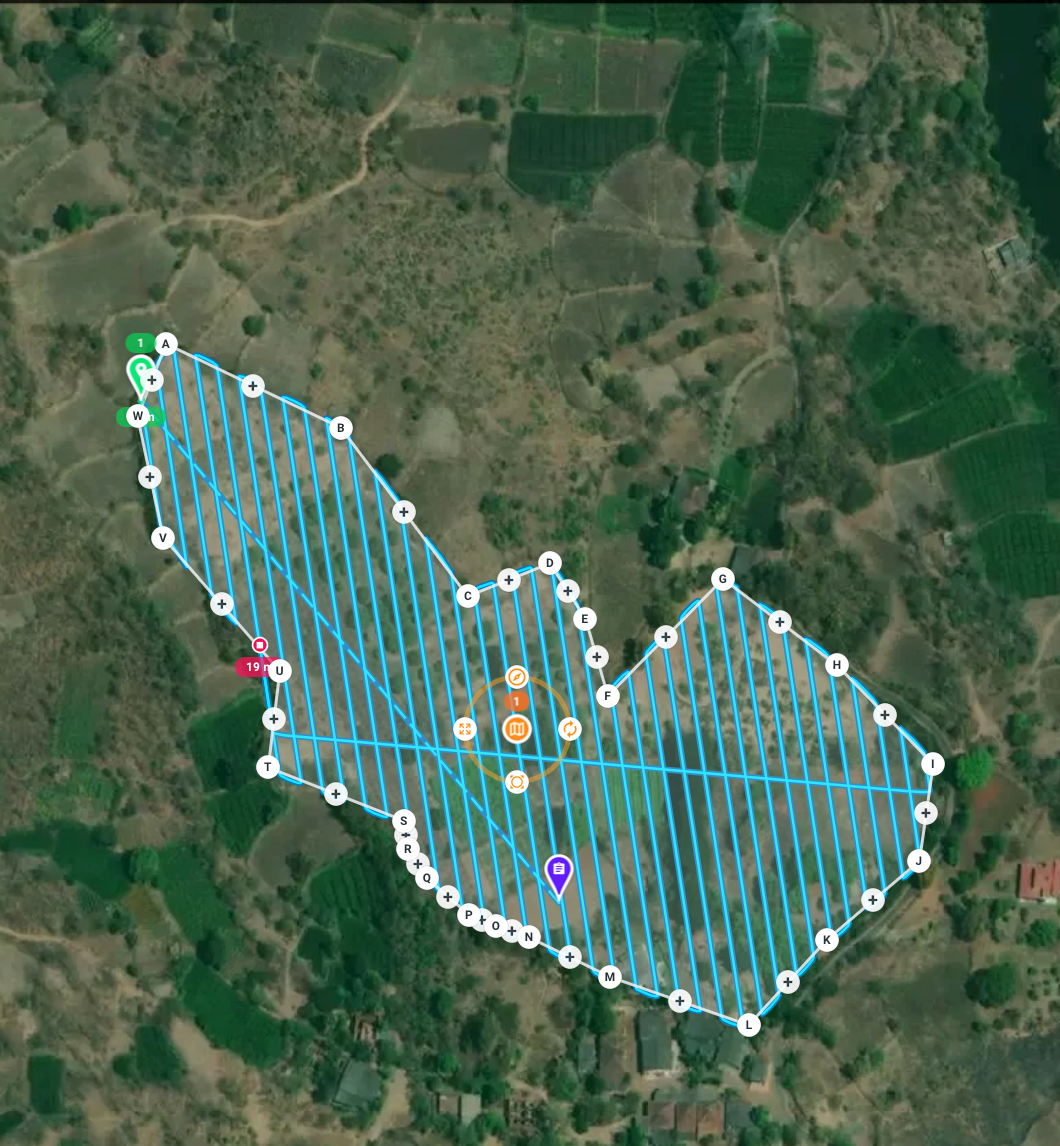
\includegraphics[width=0.5\columnwidth]{Figures/FlightPath.png}}
    \caption{Flight Path for Data Acquisition}
    \label{flightpath}
\end{figure}


\section{Methodology}

\begin{figure}[htbp]
    \centering{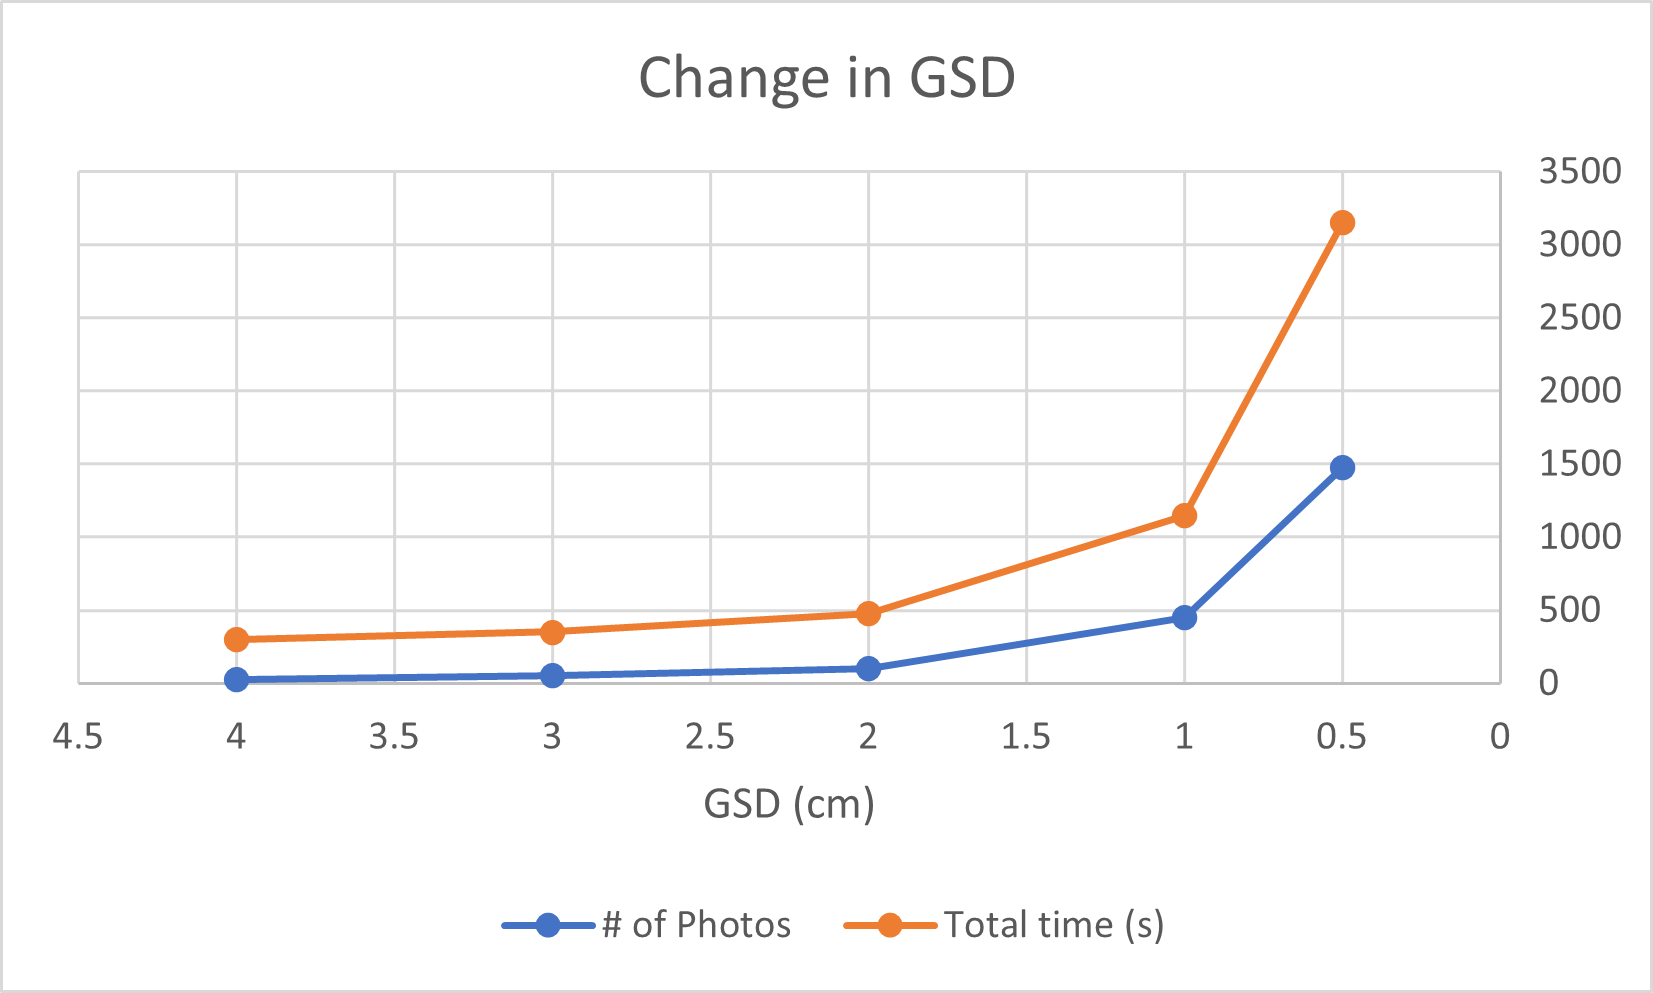
\includegraphics[width=0.8\columnwidth]{Figures/graph2.png}}
    \caption{Change in GSD}
    \label{gsd}
\end{figure}


\subsection{Data Acquisition and Study Area}

The data was acquired over a mix rural-agriculture area in
western India as shown in Figure 1 using commercial off-
the-shelf UAVs in a grid like flight path with forward and
side overlap of 90\% and 70\% respectively. Traditionally
such data is used to generate digital elevation models and
orthomosaics. It is observed that the there exists a near
exponential increase in the number of images as well as
flight time as seen in Figure 2, with an increase in ground
sampling distance or GSD (resolution) which can be
expensive in terms of time and resources. In some cases,
increasing GSD is not possible due to obstacles in flight
path at low altitude. To overcome this limitation, this paper
proposes adding a new step to the photogrammetry pipeline
as seen in Figure 3 where we use popular multimedia super-
resolution implementations to upscale raw images before
feeding them to the above-mentioned pipeline.

\begin{figure}[htbp]
    \centering{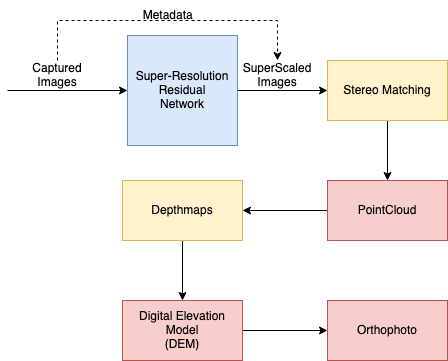
\includegraphics[width=\columnwidth]{Figures/Methodology.png}}
    \caption{Pipeline}
    \label{pipeline}
\end{figure}



\subsection{Super-Resolution and Photogrammetry}
Images captured are pre-processed and up-scaled using two
different multimedia super-resolution techniques based on
generative networks, Image Super Resolution (ISR) \cite{cardinale2018isr} and
Super-resolution Generative-Adversarial-network (SRGAN)
\cite{fastsrgan}. As seen in Figure 3, we upscale raw images captured
by the UAV using ISR and SRGAN, the up-scaled images'
metadata is modified to match that of the original image to
maintain geo-location and camera orientation information
provided by the UAV platform at the time of capture.
Up-scaled images are then processed using a mix of
commercial proprietary and open-source software to
generate digital elevation models (DEM) and orthophotos /
orthomosaics using stereo-matching and depth maps. DEMs
generated by the two methods are compared to the native-
high-resolution DEM to evaluate the performance of the
proposed technique.


\begin{figure}[htbp]
    \centering{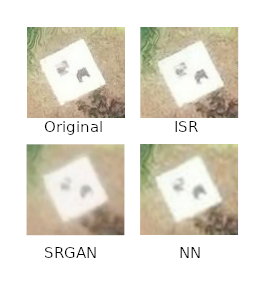
\includegraphics[width=0.75\columnwidth]{Figures/compare.png}}
    \caption{Super-Resolution Results}
    \label{compare}
\end{figure}

% \begin{center}
%     \begin{tabular}{c c c c} 
%      \hline
%      Col1 & Col2 & Col2 & Col3 \\
%     %  \hline
%      1 & 6 & 87837 & 787 \\ 
%     %  \hline
%      2 & 7 & 78 & 5415 \\
%     %  \hline
%      3 & 545 & 778 & 7507 \\
%     %  \hline
%      4 & 545 & 18744 & 7560 \\
%     %  \hline
%      5 & 88 & 788 & 6344 \\ 
%      \hline
%     \end{tabular}
% \end{center}




\setlength{\tabcolsep}{10pt} % Default value: 6pt
\renewcommand{\arraystretch}{1.5} % Default value: 1
\begin{table}[h!]
    \caption{Comparison Metrics}
    \centering
     \begin{tabular}{ c c c c c } 
     \hline
     Metric & Original & SRGAN & ISR & NN \\ [1ex] 
     \hline
     RMSE & - & 0.010 & 0.002 & 0.002 \\ 
     PSNR & - & 39.594 & 52.189 & 51.215 \\
     SSIM & - & 0.926 & 0.993 & 0.991 \\
     SIFT Density \\ (100 x 100 px) & 173.34 & 18.54 & 205.75 & 157.07 \\
     \hline
     \end{tabular}
\end{table}

Figure 4 shows the outputs of both the algorithms along
with the original image and a nearest neighbor interpolated
image. Comparative metrics have also been shown in Table 1
The next section focuses on the results and findings.

\section{Results and Discussion}

\begin{figure*}[htbp]
    \centering{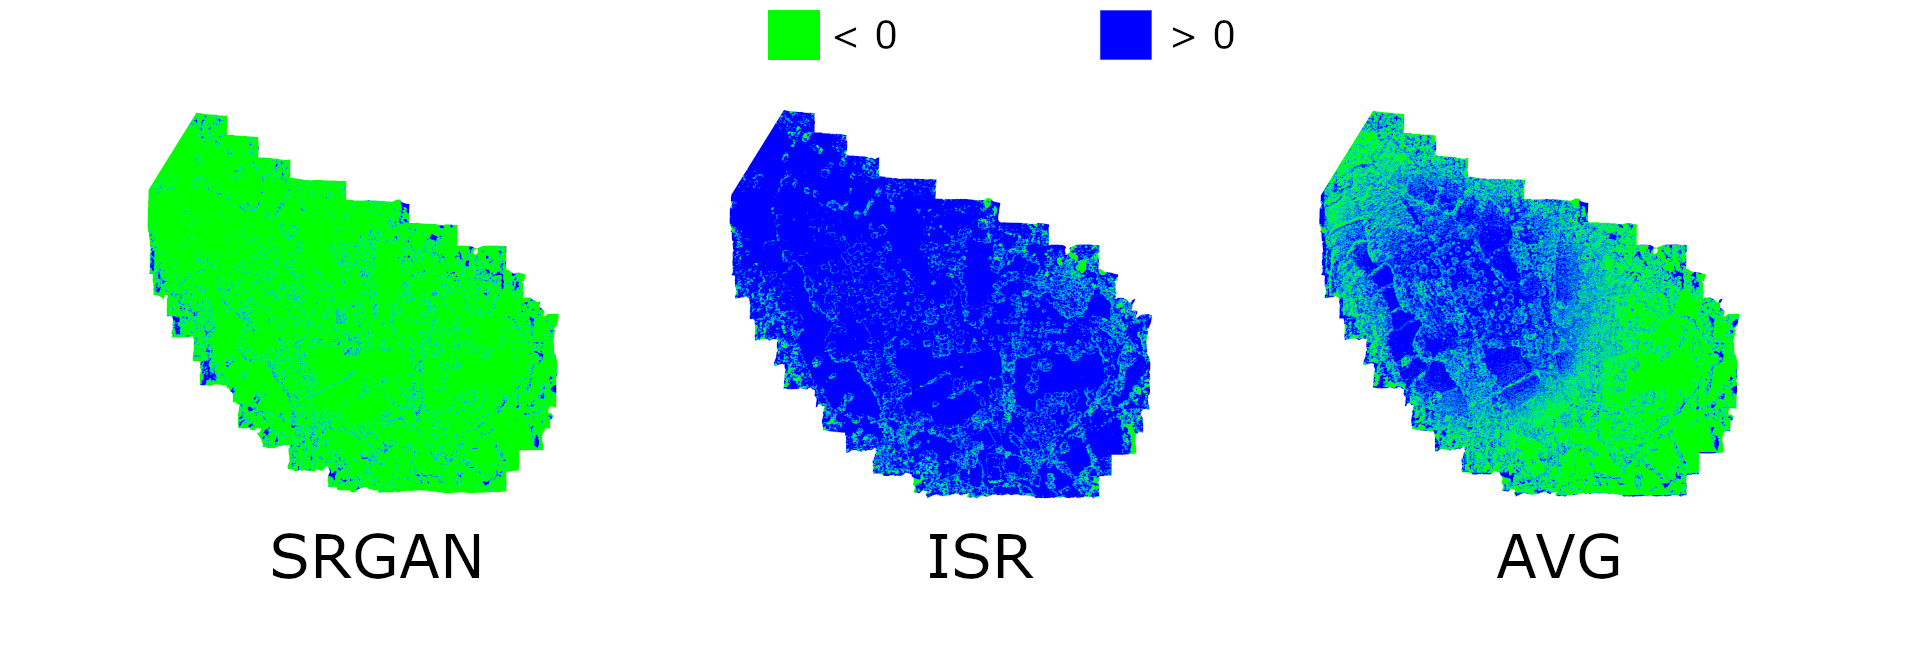
\includegraphics[width=\textwidth]{Figures/pixel.png}}
    \caption{Pixelwise elevation difference when compared with the native DEM}
    \label{span}
\end{figure*}

Digital Elevation Models (DEM) generated using each
method are evaluated against the DEM generated using
native high-resolution imagery to assess the efficacy of
using multimedia based super-resolution techniques for
UAV remote sensing. Comparison metrics include Mean
Error (ME), Root Mean Square Error (RMSE), Peak Signal
to Noise Ratio (PSNR) and Structural Similarity Index
(SSIM) where ME, RMSE and PSNR are calculated on the
DEM data structure whereas SSIM is calculated by
converting the DEMs into grayscale images.



\setlength{\tabcolsep}{10pt} % Default value: 6pt
\renewcommand{\arraystretch}{1.5} % Default value: 1
\begin{table}[h!]
    \caption{Elevation Comparison Metrics}
    \centering
     \begin{tabular}{ c c c c c } 
     \hline
     Metric & SRGAN & ISR & AVG \\ [1ex] 
     \hline
     ME (in m.) & -0.266 & 0.210 & -0.024 \\ 
     MAE (in m.) & 0.390 & 0.312 & 0.199 \\ 
     RMSE (in m.) & 0.901 & 0.733 & 0.671 \\
     PSNR & 29.95 & 31.74 & 32.51 \\
     SSIM & 0.969 & 0.977 & 0.978 \\
     \hline
     \end{tabular}
\end{table}

As seen in Table 2 it is observed that the DEM generated by
ISR shows a lower RMSE which suggests that the ISR
method produces DEMs with higher accuracy compared to
SRGAN. Likewise, PSNR, being a function of RMSE
shows comparable results. However, results become
ambiguous when it comes to ME. It is observed that the
DEM generated using SRGAN images has a negative ME
while the DEM generated by ISR images has a positive ME.
This suggests that there exists an inherent bias between the
two upscaling methods when it comes to generating DEMs
using multimedia super-resolution techniques.

According to Lillesand et. al (2004) \cite{lillesand}, for a stereoscopic
DEM generation, the elevation of a point is determined
using \\

\begin{align}
    h_{x,y}= H - \frac{B*f}{p_{x,y}}
\end{align}
h - elevation of a point \\
H - elevation of the point above a datum (usually MSL) \\
B - baseline or the distance between two stereo images \\
f - focal length of the camera \\
p - parallax / distance of the same point in two stereo images \\



To address this discrepancy, we take the DEMs generated
by both methods and generate a DEM named AVG by
shifting and averaging values from the former. It is observed
that the new DEM is more accurate, thus implying that
combining results from both methods is feasible and
effective. The efficiency of this process is assessed below.



The three DEMs image shown in Figure 5 represents the
differences between the DEMs generated using ISR and
SRGAN upscaled images as well as the combined result
AVG and the original DEM. Green pixels indicate an
undershoot in altitude estimation while blue pixels indicate
an overshoot compared to native-high-resolution DEM. The
combined DEM, AVG, gives a much better estimation and
compensates for the overshoots and undershoots. As is
evident, the values from the SRGAN method show a
negative bias while the values belonging to ISR show a
positive bias. The combination of the two (Averaging)
produces results that close to the original. 

\begin{figure}[htbp]
    \centering{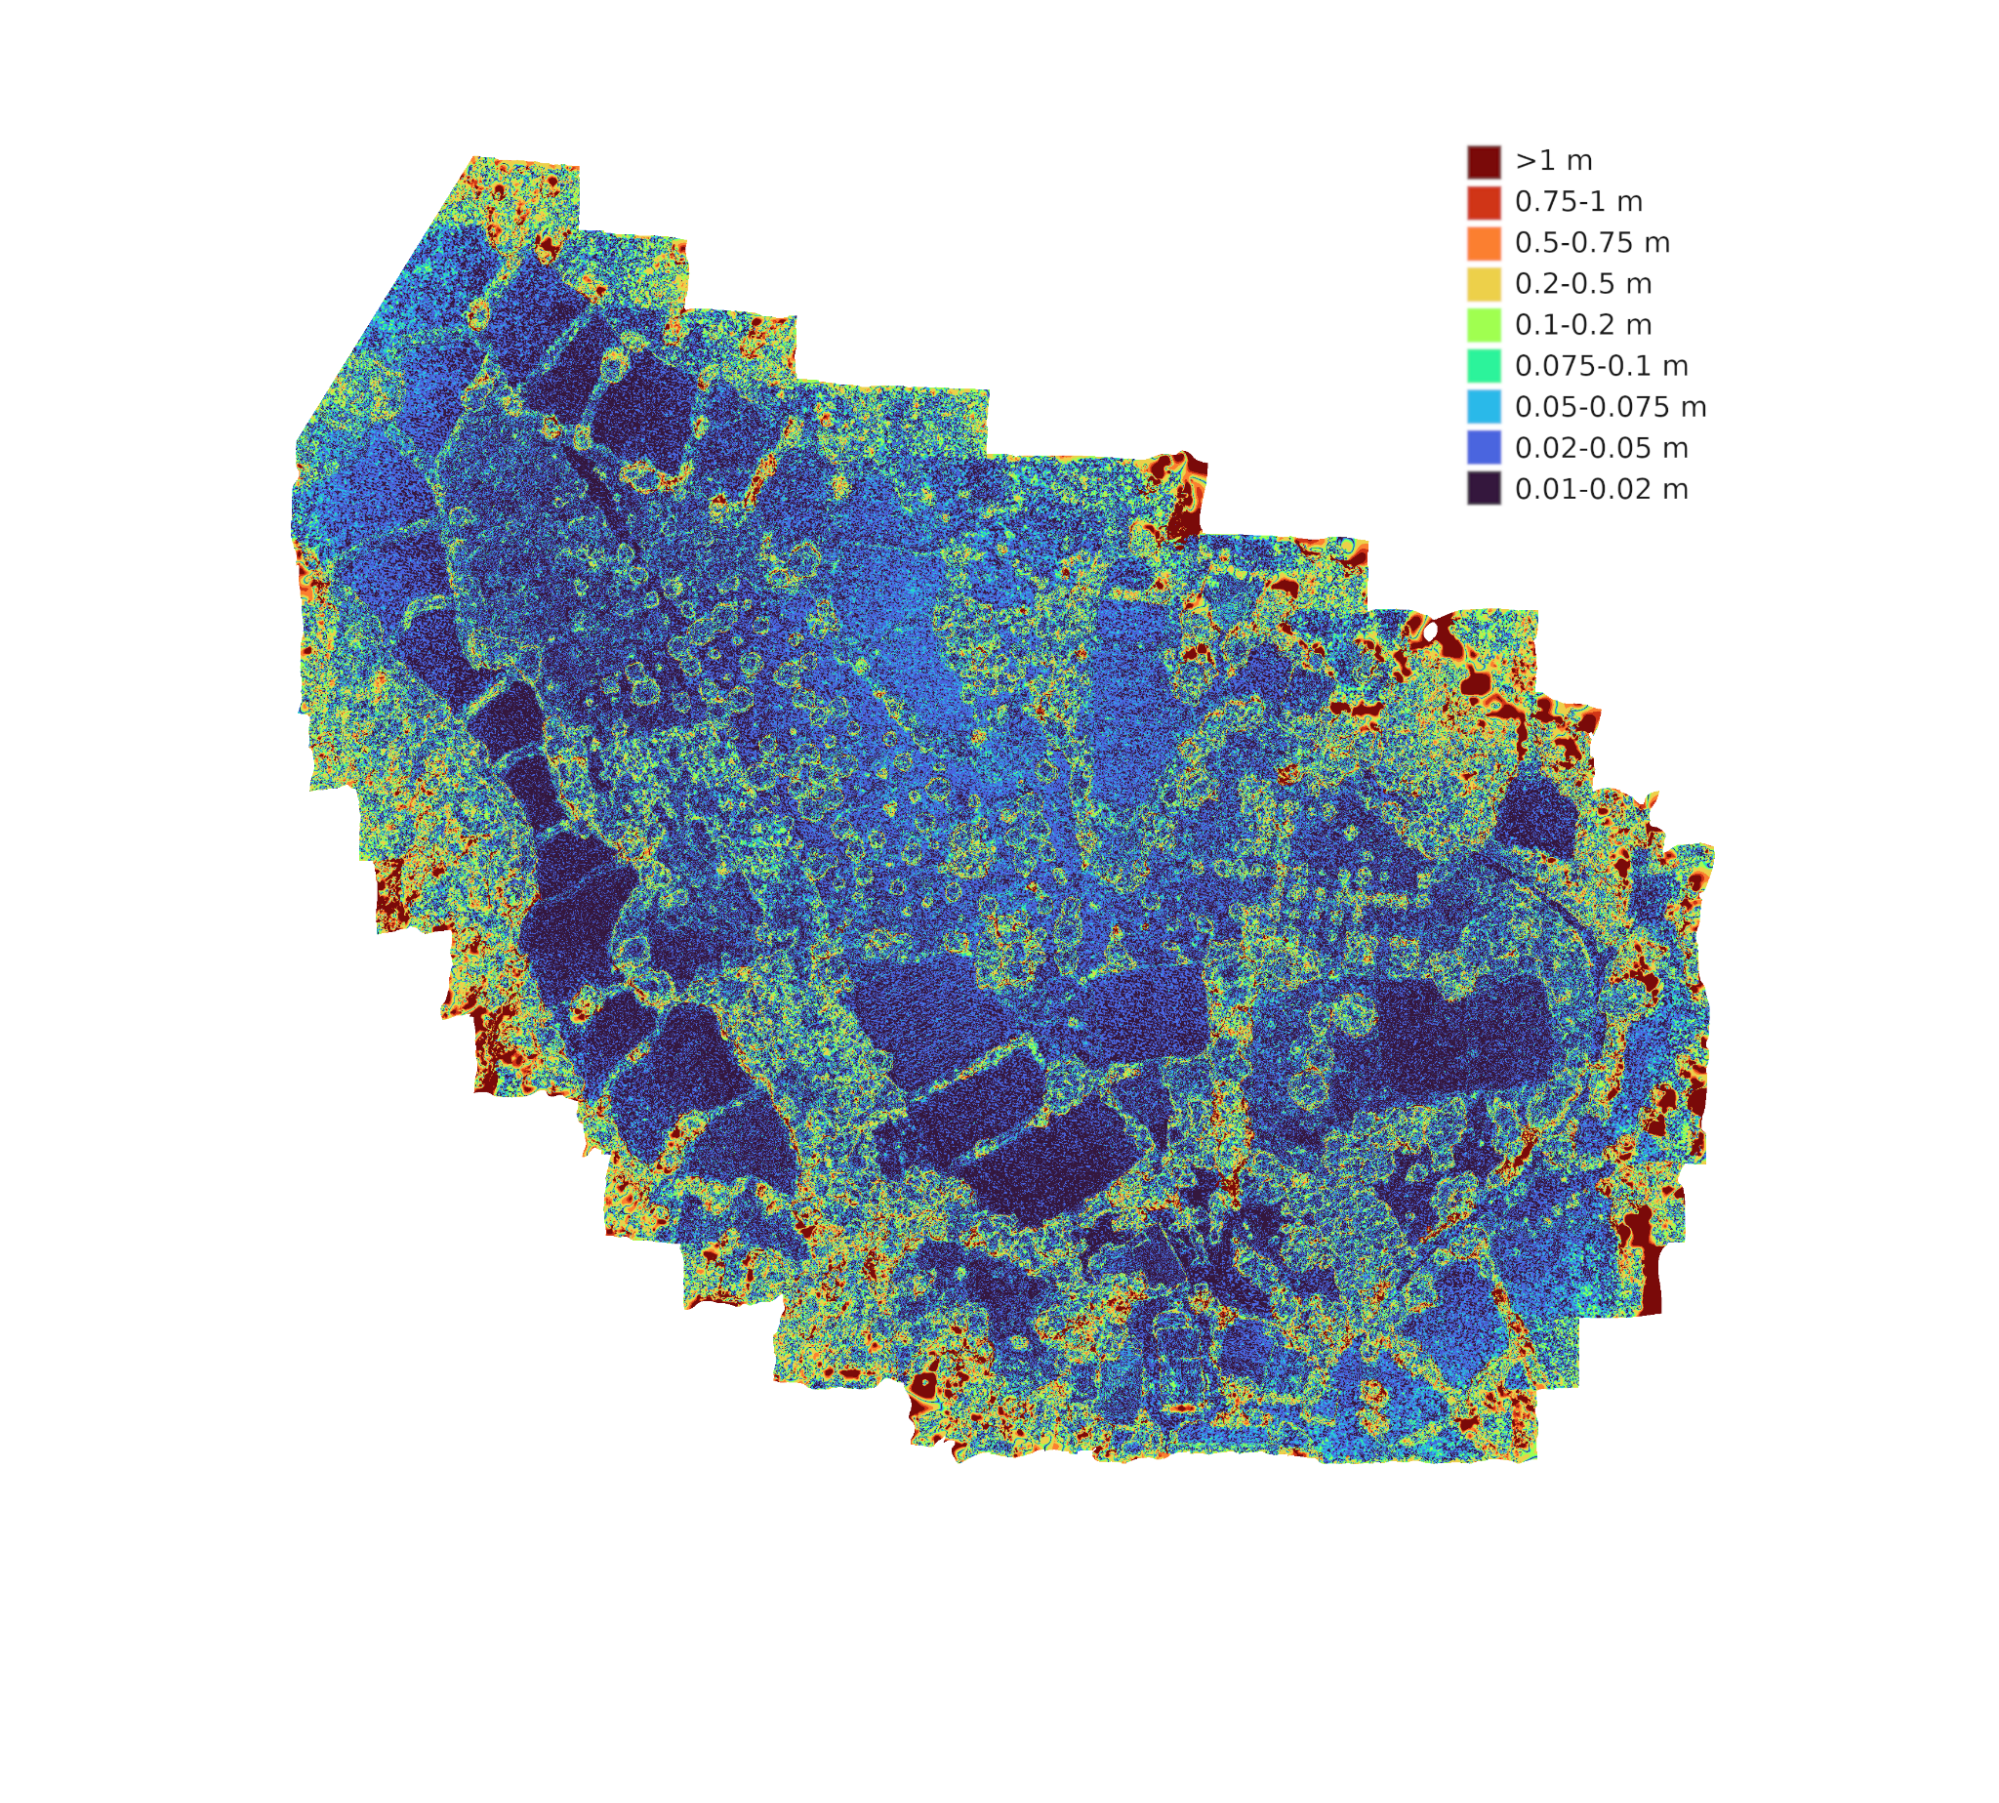
\includegraphics[width=0.8\columnwidth]{Figures/avg.png}}
    \caption{Absolute Elevation Difference}
    \label{avg}
\end{figure}


Figure 6 is the absolute elevation difference between the averaged DEM
compared to original. An overall increase in accuracy is
observed with the large blue patches indicating small errors.

\section{Concusion}
Generating High-Resolution Digital Elevation Models
(HRDEM) from Low-Resolution Digital Elevation Models
(LRDEM) has been previously studied using traditional
interpolation techniques as well as modern approaches like
neural networks which tend to have an added benefit of
learning certain patterns and approximating them with high
fidelity. However, in this paper we generate HRDEMs from
super resolved images in contrast to upscaling the elevation
models. From the results it is evident that using multimedia
super-resolution techniques to generate DEMs from low-
resolution images can result in HRDEMs that have a small
bias. Additionally, combining the results from the two
methods can result in a HRDEM that is more accurate.
Further research can include tuning the generative network
for specific use to improve DEM accuracy and decrease
processing time.

% \subsection{Units}
% \begin{itemize}
% \item Use either SI (MKS) or CGS as primary units. (SI units are encouraged.) English units may be used as secondary units (in parentheses). An exception would be the use of English units as identifiers in trade, such as ``3.5-inch disk drive''.
% \item Avoid combining SI and CGS units, such as current in amperes and magnetic field in oersteds. This often leads to confusion because equations do not balance dimensionally. If you must use mixed units, clearly state the units for each quantity that you use in an equation.
% \item Do not mix complete spellings and abbreviations of units: ``Wb/m\textsuperscript{2}'' or ``webers per square meter'', not ``webers/m\textsuperscript{2}''. Spell out units when they appear in text: ``. . . a few henries'', not ``. . . a few H''.
% \item Use a zero before decimal points: ``0.25'', not ``.25''. Use ``cm\textsuperscript{3}'', not ``cc''.)
% \end{itemize}

% \subsection{Equations}
% Number equations consecutively. To make your 
% equations more compact, you may use the solidus (~/~), the exp function, or 
% appropriate exponents. Italicize Roman symbols for quantities and variables, 
% but not Greek symbols. Use a long dash rather than a hyphen for a minus 
% sign. Punctuate equations with commas or periods when they are part of a 
% sentence, as in:
% \begin{equation}
% a+b=\gamma\label{eq}
% \end{equation}

% Be sure that the 
% symbols in your equation have been defined before or immediately following 
% the equation. Use ``\eqref{eq}'', not ``Eq.~\eqref{eq}'' or ``equation \eqref{eq}'', except at 
% the beginning of a sentence: ``Equation \eqref{eq} is . . .''

% \subsection{\LaTeX-Specific Advice}

% Please use ``soft'' (e.g., \verb|\eqref{Eq}|) cross references instead
% of ``hard'' references (e.g., \verb|(1)|). That will make it possible
% to combine sections, add equations, or change the order of figures or
% citations without having to go through the file line by line.

% Please don't use the \verb|{eqnarray}| equation environment. Use
% \verb|{align}| or \verb|{IEEEeqnarray}| instead. The \verb|{eqnarray}|
% environment leaves unsightly spaces around relation symbols.

% Please note that the \verb|{subequations}| environment in {\LaTeX}
% will increment the main equation counter even when there are no
% equation numbers displayed. If you forget that, you might write an
% article in which the equation numbers skip from (17) to (20), causing
% the copy editors to wonder if you've discovered a new method of
% counting.

% {\BibTeX} does not work by magic. It doesn't get the bibliographic
% data from thin air but from .bib files. If you use {\BibTeX} to produce a
% bibliography you must send the .bib files. 

% {\LaTeX} can't read your mind. If you assign the same label to a
% subsubsection and a table, you might find that Table I has been cross
% referenced as Table IV-B3. 

% {\LaTeX} does not have precognitive abilities. If you put a
% \verb|\label| command before the command that updates the counter it's
% supposed to be using, the label will pick up the last counter to be
% cross referenced instead. In particular, a \verb|\label| command
% should not go before the caption of a figure or a table.

% Do not use \verb|\nonumber| inside the \verb|{array}| environment. It
% will not stop equation numbers inside \verb|{array}| (there won't be
% any anyway) and it might stop a wanted equation number in the
% surrounding equation.

% \subsection{Some Common Mistakes}\label{SCM}
% \begin{itemize}
% \item The word ``data'' is plural, not singular.
% \item The subscript for the permeability of vacuum $\mu_{0}$, and other common scientific constants, is zero with subscript formatting, not a lowercase letter ``o''.
% \item In American English, commas, semicolons, periods, question and exclamation marks are located within quotation marks only when a complete thought or name is cited, such as a title or full quotation. When quotation marks are used, instead of a bold or italic typeface, to highlight a word or phrase, punctuation should appear outside of the quotation marks. A parenthetical phrase or statement at the end of a sentence is punctuated outside of the closing parenthesis (like this). (A parenthetical sentence is punctuated within the parentheses.)
% \item A graph within a graph is an ``inset'', not an ``insert''. The word alternatively is preferred to the word ``alternately'' (unless you really mean something that alternates).
% \item Do not use the word ``essentially'' to mean ``approximately'' or ``effectively''.
% \item In your paper title, if the words ``that uses'' can accurately replace the word ``using'', capitalize the ``u''; if not, keep using lower-cased.
% \item Be aware of the different meanings of the homophones ``affect'' and ``effect'', ``complement'' and ``compliment'', ``discreet'' and ``discrete'', ``principal'' and ``principle''.
% \item Do not confuse ``imply'' and ``infer''.
% \item The prefix ``non'' is not a word; it should be joined to the word it modifies, usually without a hyphen.
% \item There is no period after the ``et'' in the Latin abbreviation ``et al.''.
% \item The abbreviation ``i.e.'' means ``that is'', and the abbreviation ``e.g.'' means ``for example''.
% \end{itemize}
% An excellent style manual for science writers is \cite{b7}.

% \subsection{Authors and Affiliations}
% \textbf{The class file is designed for, but not limited to, six authors.} A 
% minimum of one author is required for all conference articles. Author names 
% should be listed starting from left to right and then moving down to the 
% next line. This is the author sequence that will be used in future citations 
% and by indexing services. Names should not be listed in columns nor group by 
% affiliation. Please keep your affiliations as succinct as possible (for 
% example, do not differentiate among departments of the same organization).

% \subsection{Identify the Headings}
% Headings, or heads, are organizational devices that guide the reader through 
% your paper. There are two types: component heads and text heads.

% Component heads identify the different components of your paper and are not 
% topically subordinate to each other. Examples include Acknowledgments and 
% References and, for these, the correct style to use is ``Heading 5''. Use 
% ``figure caption'' for your Figure captions, and ``table head'' for your 
% table title. Run-in heads, such as ``Abstract'', will require you to apply a 
% style (in this case, italic) in addition to the style provided by the drop 
% down menu to differentiate the head from the text.

% Text heads organize the topics on a relational, hierarchical basis. For 
% example, the paper title is the primary text head because all subsequent 
% material relates and elaborates on this one topic. If there are two or more 
% sub-topics, the next level head (uppercase Roman numerals) should be used 
% and, conversely, if there are not at least two sub-topics, then no subheads 
% should be introduced.

% \subsection{Figures and Tables}
% \paragraph{Positioning Figures and Tables} Place figures and tables at the top and 
% bottom of columns. Avoid placing them in the middle of columns. Large 
% figures and tables may span across both columns. Figure captions should be 
% below the figures; table heads should appear above the tables. Insert 
% figures and tables after they are cited in the text. Use the abbreviation 
% ``Fig.~\ref{fig}'', even at the beginning of a sentence.

% \begin{table}[htbp]
% \caption{Table Type Styles}
% \begin{center}
% \begin{tabular}{|c|c|c|c|}
% \hline
% \textbf{Table}&\multicolumn{3}{|c|}{\textbf{Table Column Head}} \\
% \cline{2-4} 
% \textbf{Head} & \textbf{\textit{Table column subhead}}& \textbf{\textit{Subhead}}& \textbf{\textit{Subhead}} \\
% \hline
% copy& More table copy$^{\mathrm{a}}$& &  \\
% \hline
% \multicolumn{4}{l}{$^{\mathrm{a}}$Sample of a Table footnote.}
% \end{tabular}
% \label{tab1}
% \end{center}
% \end{table}

% \begin{figure}[htbp]
% \centerline{
\includegraphics{fig1.png}}
% \caption{Example of a figure caption.}
% \label{fig}
% \end{figure}

% Figure Labels: Use 8 point Times New Roman for Figure labels. Use words 
% rather than symbols or abbreviations when writing Figure axis labels to 
% avoid confusing the reader. As an example, write the quantity 
% ``Magnetization'', or ``Magnetization, M'', not just ``M''. If including 
% units in the label, present them within parentheses. Do not label axes only 
% with units. In the example, write ``Magnetization (A/m)'' or ``Magnetization 
% \{A[m(1)]\}'', not just ``A/m''. Do not label axes with a ratio of 
% quantities and units. For example, write ``Temperature (K)'', not 
% ``Temperature/K''.

% \section*{Acknowledgment}

% The preferred spelling of the word ``acknowledgment'' in America is without 
% an ``e'' after the ``g''. Avoid the stilted expression ``one of us (R. B. 
% G.) thanks $\ldots$''. Instead, try ``R. B. G. thanks$\ldots$''. Put sponsor 
% acknowledgments in the unnumbered footnote on the first page.

% \section*{References}

% Please number citations consecutively within brackets \cite{b1}. The 
% sentence punctuation follows the bracket \cite{b2}. Refer simply to the reference 
% number, as in \cite{b3}---do not use ``Ref. \cite{b3}'' or ``reference \cite{b3}'' except at 
% the beginning of a sentence: ``Reference \cite{b3} was the first $\ldots$''

% Number footnotes separately in superscripts. Place the actual footnote at 
% the bottom of the column in which it was cited. Do not put footnotes in the 
% abstract or reference list. Use letters for table footnotes.

% Unless there are six authors or more give all authors' names; do not use 
% ``et al.''. Papers that have not been published, even if they have been 
% submitted for publication, should be cited as ``unpublished'' \cite{b4}. Papers 
% that have been accepted for publication should be cited as ``in press'' \cite{b5}. 
% Capitalize only the first word in a paper title, except for proper nouns and 
% element symbols.

% For papers published in translation journals, please give the English 
% citation first, followed by the original foreign-language citation \cite{b6}.
\bibliographystyle{IEEEtran}
\bibliography{References/Gen}
\end{document}
